%Master File:lectures.tex

\lesson{Over-Fitting}
\vspace{-1cm}
\begin{center}
\includegraphics[width=0.45\linewidth]{tiger6} \hfill
\includegraphics[width=0.45\linewidth]{wolf6}
\end{center}
\keywords{Overfitting, regularisation, feature selection}
%%%%%%%%%%%%%%%%%%%%%%% Next Slide %%%%%%%%%%%%%%%%%%%%%%%
\renewcommand{\Outline}{%
\begin{slide}
\section[1]{Outline}

\begin{minipage}{12cm}\raggedright
  \begin{enumerate}\squeeze
    \outlineitem{Over-fitting?}{overfitting}
    \outlineitem{Controlling Complexity}{complexity}
    \outlineitem{Hidden structure}{hidden}
    \outlineitem{Regularisation}{regularisers}
  \end{enumerate}
\end{minipage}\hfill
\begin{minipage}{10cm}
  \includegraphics[width=10cm]{tiger1.jpg}
\end{minipage}
\end{slide}
\addtocounter{outlineitem}{1}
}

\setcounter{outlineitem}{1}

%%%%%%%%%%%%%%%%%%%%%%% Next Slide %%%%%%%%%%%%%%%%%%%%%%%
\Outline % Why ML works
\toptarget{firstoutline}
%%%%%%%%%%%%%%%%%%%%%%% Next Slide %%%%%%%%%%%%%%%%%%%%%%%

\begin{slide}
\section{Over-fitting}

\begin{PauseHighLight}
  \begin{itemize}
  \item Complex machine can \emph{over-fitting}
    \begin{quote}
      \textit{\textbf{over-fitting}: fitting the training data well at
        the cost of getting poorer generalisation performance}\pause
    \end{quote}
  \item Three red cars\ldots\pause
  \item If we used an infinitely flexible machine we can fit our
    training data perfectly, but would have no generalisation
    ability\pause
  \end{itemize}
\end{PauseHighLight}

\end{slide}

%%%%%%%%%%%%%%%%%%%%%%% Next Slide %%%%%%%%%%%%%%%%%%%%%%%

\begin{slide}
\section[-2]{Binary Classification Task for You}

\begin{center}
  \setlength{\unitlength}{1mm}
  \begin{picture}(240,150)
    \put(115,-5){\line(0,1){145}}
    \put(114,-5){\line(0,1){145}}
    \put(116,-5){\line(0,1){145}}
    \put(0,0){\includegraphics[width=5cm]{tiger4.png}}
    \put(60,0){\includegraphics[width=5cm]{tiger5.png}}
    \put(0,50){\includegraphics[width=5cm]{tiger6.png}}
    \put(60,50){\includegraphics[width=5cm]{tiger7.png}}
    \put(0,100){\includegraphics[width=5cm]{tiger8.png}}
    \put(60,100){\includegraphics[width=5cm]{tiger9.png}}
    \put(120,0){\includegraphics[width=5cm]{wolf1.png}}
    \put(180,0){\includegraphics[width=5cm]{wolf2.png}}
    \put(120,50){\includegraphics[width=5cm]{wolf3.png}}
    \put(180,50){\includegraphics[width=5cm]{wolf4.png}}
    \put(120,100){\includegraphics[width=5cm]{wolf5.png}}
    \put(180,100){\includegraphics[width=5cm]{wolf6.png}}
    \put(55,-5){\makebox(0,0){Class 1}}
    \put(175,-5){\makebox(0,0){Class 2}}
  \end{picture}
\end{center}

\end{slide}



%%%%%%%%%%%%%%%%%%%%%%% Next Slide %%%%%%%%%%%%%%%%%%%%%%%

\begin{slide}
\section{Which Category?}

\begin{PauseHighLight}
  \begin{itemize}
  \item Which category does the following image belong to?
    \begin{center}
      \includegraphics[height=10cm]{tiger1.jpg}
    \end{center}
  \end{itemize}
\end{PauseHighLight}

\end{slide}

%%%%%%%%%%%%%%%%%%%%%%% Next Slide %%%%%%%%%%%%%%%%%%%%%%%

\begin{slide}
\section{Spurious Rules}

\begin{PauseHighLight}
  \begin{itemize}
  \item You ask a learning machine to solve a task based on data\pause
  \item It will find a rule that does this, but not necessary the rule
    you had in mind\pause---machine learning isn't magic, it can't
    read your mind\pauseb
  \item Infinitely flexible machines have an infinity of spurious
    rules they can learn\pause---they are useless\pauseb
  \item What should we do?\pause
  \end{itemize}
\end{PauseHighLight}

\end{slide}

%%%%%%%%%%%%%%%%%%%%%%% Next Slide %%%%%%%%%%%%%%%%%%%%%%%

\begin{slide}
\section[-2]{All Binary Functions}

\pb \pause \pauselevel{=1}
\begin{center}
  \multipdf[width=\linewidth]{flexibleMachine}\pause
\end{center}
\end{slide}

%%%%%%%%%%%%%%%%%%%%%%% Next Slide %%%%%%%%%%%%%%%%%%%%%%%

\begin{slide}
\section{Are MLPs Universal Approximators?}

\begin{PauseHighLight}
  \begin{itemize}
  \item Yes\pauseb{} and No\pauseb
  \item Yes: If you give me any function, I can find an MLP that
    approximates that function to any desired accuracy\pauseb
  \item No: If you give me an MLP, I can find a function with an
    arbitrary high approximation error\pauseb
  \item Would an MLP that could approximate any function be
    useful?\pauseb
  \item \emph{Absolutely not!}\pauseb
  \end{itemize}
\end{PauseHighLight}

\end{slide}



%%%%%%%%%%%%%%%%%%%%%%% Next Slide %%%%%%%%%%%%%%%%%%%%%%%
\Outline % Controlling Complexity
%%%%%%%%%%%%%%%%%%%%%%% Next Slide %%%%%%%%%%%%%%%%%%%%%%%

\begin{slide}
\section{Controlling Complexity}

\begin{PauseHighLight}
  \begin{itemize}
  \item Infinitely flexible machine don't generalise\pause{} (because
    any unseen data could have any value)\pauseb
  \item \emph{Machine learning only works because we believe there is
      some structure in the data}\pause
  \item A successful machine should capture this structure\pause
  \item Even deep learning machines with millions of parameters only
    work because they successfully capture the structure of images or
    text\pause
  \item Different learning machines have different performance on
    different problems because the data has different structure\pause
  \end{itemize}
\end{PauseHighLight}

\end{slide}


%%%%%%%%%%%%%%%%%%%%%%% Next Slide %%%%%%%%%%%%%%%%%%%%%%%


\begin{slide}
\section{Training Examples}

\begin{PauseHighLight}
  \begin{itemize}
  \item As we increase the number of training examples, we make it hard
    to find a spurious rule\pause
  \item Bigger data sets allow us to use more complicated
    machines\pause
  \item Part of the success of deep learning is because they use huge
    training sets\pause---but this is only a part of their success\pauseb
  \item (Labelled) data is often expensive to collect so we
    sometimes have no choice but to use a small training set\pause
  \item One of the limitations of using deep learning comes because we often
    have limited data\pause
  \end{itemize}
\end{PauseHighLight}

\end{slide}


%%%%%%%%%%%%%%%%%%%%%%% Next Slide %%%%%%%%%%%%%%%%%%%%%%%

\begin{slide}
\section{Identifying Structure}

\begin{PauseHighLight}
  \begin{itemize}
  \item In some cases we know \textit{a priori} some of the structure
    in the data\pause
  \item In images we believe the identity of an object is invariant to
    translation and scaling\pause
  \item The success of \textit{convolutional neural networks} (CNNs)
    in deep learning is in large part because the convolutions respect
    translational invariance\pause
  \item The position of words in a sentence does not change its
    meaning (it might change the meaning of the sentence) and CNNs are
    often successful in understanding text\pause
  \end{itemize}
\end{PauseHighLight}

\end{slide}

%%%%%%%%%%%%%%%%%%%%%%% Next Slide %%%%%%%%%%%%%%%%%%%%%%%

\begin{slide}
\section{Preprocessing}

\begin{PauseHighLight}
  \begin{itemize}
  \item Structure might often be obscure to the learning machine\pause
  \item If we are trying to predict the spread of disease then a list
    of place names might be a lot less useful than their
    coordinates\pause
  \item Imposing an ordering on an unordered set might not be useful
    \begin{align*}
      \left\{\strut \text{``blue''}:0,\;\text{``brown''}:1,\;
      \text{``green''}:2,\;\text{``black''}:3 \right\}\pause
    \end{align*}
  \item Choosing an encoding that reflect meaningful structure is
    essential to successful machine learning\pause
  \end{itemize}
\end{PauseHighLight}

\end{slide}

%%%%%%%%%%%%%%%%%%%%%%% Next Slide %%%%%%%%%%%%%%%%%%%%%%%

\begin{slide}
\section[-2]{Automatic Preprocessing}

\begin{PauseHighLight}
  \begin{itemize}
  \item One view of deep learning is that each layer (particularly in
    CNNs) acts as a preprocessor\pause
  \item That is, it finds filters that captures features salient to
    the problem being tackled\pause
  \item For both images and texts we expect salient features to be
    spatially localised\pause{} (CNN finds localised filter)\pauseb 
  \item The deep structure allows ever more complicated features to be
    captured---that is, we can find spatially localised features on
    different scales\pause
  \item Having very large datasets and simple filters (the number of
    weights in the CNN layers tends to be small) stops
    overfitting\pause
  \end{itemize}
\end{PauseHighLight}

\end{slide}




%%%%%%%%%%%%%%%%%%%%%%% Next Slide %%%%%%%%%%%%%%%%%%%%%%%
\Outline % Hidden structure
%%%%%%%%%%%%%%%%%%%%%%% Next Slide %%%%%%%%%%%%%%%%%%%%%%%

\begin{slide}
  \section{Hidden Structure}

  \begin{PauseHighLight}
    \begin{itemize}
    \item Often the structure of data is invisible to us\pause
    \item A very successful strategy is to try many different machine
      learning techniques and choose the best\pause{} (stupid but
      effective)\pauseb
    \item Often learning machines have adjustable parameters
      (hyper-parameters) that we have to set (they are the same for
      all input data, but change with the problem)\pause
    \item We need to choose the hyper-parameters to fit the data in
      our problem\pause
    \item Fine tuning hyper-parameter is important\pause{} and almost always
      required (true in SVMs, MLP, deep learning)\pauseb
    \end{itemize}
  \end{PauseHighLight}

\end{slide}

%%%%%%%%%%%%%%%%%%%%%%% Next Slide %%%%%%%%%%%%%%%%%%%%%%%

\begin{slide}
\section{Measuring Generalisation Performance}

\begin{PauseHighLight}
  \begin{itemize}
  \item Recall, we want to predict \emph{unseen} data\pause
  \item \emph{You cannot use data that you have trained
      on!}\pause---you will overfit\pauseb
  \item Need to split your data up into training and validation
    set\pause
  \item Use the validation set to choose the hyper-parameters\pause
  \item You need a separate testing set if you want to measure your
    generalisation performance\pause
  \end{itemize}
\end{PauseHighLight}

\end{slide}

%%%%%%%%%%%%%%%%%%%%%%% Next Slide %%%%%%%%%%%%%%%%%%%%%%%

\begin{slide}
\section[-2]{The Overfitting Game}

\pb\pause\pauselevel{=1}
\begin{center}
  \multipdf[width=\linewidth]{overfit}\pause
\end{center}

\end{slide}



%%%%%%%%%%%%%%%%%%%%%%% Next Slide %%%%%%%%%%%%%%%%%%%%%%%

\begin{slide}
  \section[-2]{Cross Validation}
  
\pb
\begin{itemize}
\item If you want to use more data for training then you can use cross
  validation\pauseh
\item $K$-fold cross validation splits the data into $K$ groups\pauseh
\end{itemize}
\begin{center}
  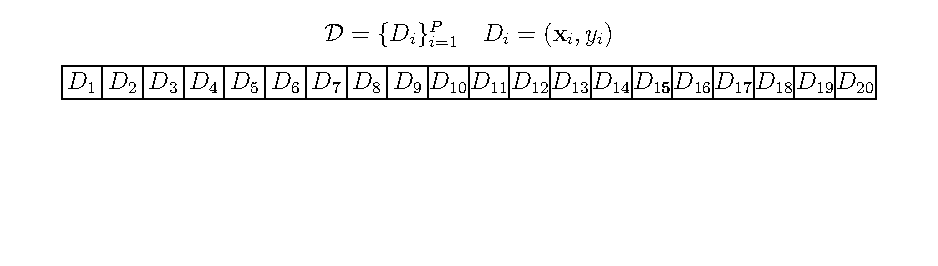
\includegraphics[width=0.9\linewidth]{cross_validation0}\mypl{1 :3}
  \multido{\ia=1+1,\ib=4+1}{23}{%
    \llap{\includegraphics[width=0.9\linewidth]{cross_validation\ia}}\mypl{\ib}}
  \llap{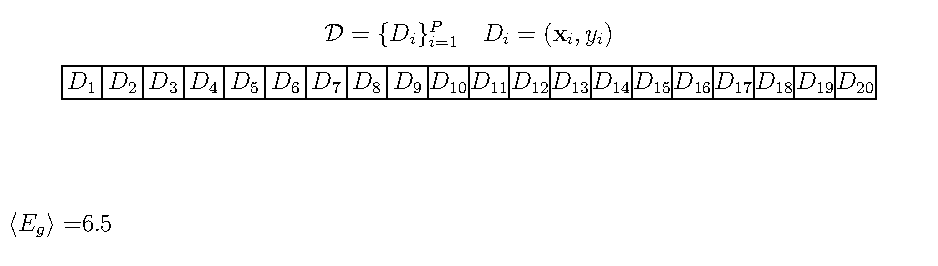
\includegraphics[width=0.9\linewidth]{cross_validation23}}
\end{center}
\begin{itemize}
\item Leave-one-out cross-validation is extreme case\pause
\end{itemize}
\end{slide}



%%%%%%%%%%%%%%%%%%%%%%% Next Slide %%%%%%%%%%%%%%%%%%%%%%%

\begin{slide}
\section[-2]{Hidden Structure}

\pb
Can't spot low dimensional data by looking at numbers\pause
\begin{center}
  \includegraphics[width=0.7\linewidth]{rotate3d0}\mypl{1}
  \multido{\ia=1+1,\ib=2+1}{6}{%
    \llap{\includegraphics[width=0.7\linewidth]{rotate3d\ia}}\mypl{\ib}}
\end{center}

\end{slide}


%%%%%%%%%%%%%%%%%%%%%%% Next Slide %%%%%%%%%%%%%%%%%%%%%%%

\begin{slide}
\section{Dimensionality Reduction}

\begin{PauseHighLight}
  \begin{itemize}
  \item We can sometimes simplify our machines by using less features\pause
  \item We can project our data onto a lower dimensional sub-space
    (e.g. one with the maximum variation in the data: PCA)\pause
  \item We can use clustering to find exemplars and recode our data in
    terms of distances from the exemplars (radial basis
    functions)\pause
  \item Whether this helps depends on whether the information we discard
    is pertinent to the task we are trying to perform\pause
  \end{itemize}
\end{PauseHighLight}

\end{slide}



%%%%%%%%%%%%%%%%%%%%%%% Next Slide %%%%%%%%%%%%%%%%%%%%%%%

\begin{slide}
\section[-1]{Feature Selection}

\begin{PauseHighLight}
  \begin{itemize}
  \item Spurious features will allow us to find spurious rules
    (\emph{over-fitting})\pause
  \item We can try different combinations of features to find the best
    set, although it rapidly becomes intractable to do this in all
    ways\pause
  \item We can use various heuristics to decide which features to keep,
    but no heuristic is fail-safe method to find the best set of features\pause
  \item Feature selection however can be powerful, often we can get very
    good results by keeping only a few variables\pause
  \item As well as possibly improving generalisation we also get a more
    \emph{interpretable} rule\pause
  \end{itemize}
\end{PauseHighLight}

\end{slide}

%%%%%%%%%%%%%%%%%%%%%%% Next Slide %%%%%%%%%%%%%%%%%%%%%%%

\begin{slide}
\section{Normalising Features}

\begin{PauseHighLight}
  \begin{itemize}
  \item Measuring a feature in millimeters or kilometers is going
    to make a lot of difference to the size of that feature\pause
  \item Many learning algorithms are sensitive to the size of a
    feature (larger features are more important)\pause
  \item If we don't know how important different features are then it
    makes sense to normalise our features\pause, E.g.
    \begin{align*}
      x^\alpha_i &\leftarrow \frac{x^\alpha_i-\hat{\mu}_i}{\hat{\sigma}_i},
      &
      \hat{\mu} &= \frac{1}{m} \sum_{\beta=1}^m x_i^\beta,
      &
      \hat{\sigma}_i^2 &= \frac{1}{m-1} \sum_{\beta=1}^m
                       (x_i^\beta-\hat{\mu}_i)^2\pauseb 
    \end{align*}
  \end{itemize}
\end{PauseHighLight}

\end{slide}




%%%%%%%%%%%%%%%%%%%%%%% Next Slide %%%%%%%%%%%%%%%%%%%%%%%
\Outline % Regularisation
%%%%%%%%%%%%%%%%%%%%%%% Next Slide %%%%%%%%%%%%%%%%%%%%%%%

\begin{slide}
\section[-2]{Explicit Regularisation}

\begin{PauseHighLight}
  \begin{itemize}
  \item As you've seen in the foundations of ML course, we can modify
    our error function to choose smoother functions
    \begin{align*}
      E = \sum_{k=1}^m \left( \bm{w}^\tr \, \bm{x}_k - y_k \right)^2\pause
      + \nu \, \|\bm{w}\|^2\pauseb
    \end{align*}
    (Good to normalise features)\pauseb
  \item Second term is minimised when $w_i=0$\pause
  \item If $w_i$ is large then
    \begin{align*}
      f(\bm{x}|\bm{w})= \bm{w}^\tr \, \bm{x}_n\pause = \sum_{j=1}^p
      w_j\,x_j\pauseb
    \end{align*}
    varies rapidly as we change $x_i$\pause    
  \end{itemize}
\end{PauseHighLight}

\end{slide}

%%%%%%%%%%%%%%%%%%%%%%% Next Slide %%%%%%%%%%%%%%%%%%%%%%%

\begin{slide}
\section[-2.5]{Lasso}

\pb
\begin{itemize}\squeeze
\item We can us other regularisers
  \begin{align*}
    E = \sum_{k=1}^m \left( \bm{w}^\tr \, \bm{x}_k - y_k \right)^2\pauseh
    + \nu \, \sum_{i=1}^p |w_i| \pauseb
  \end{align*}
\item Spurious features (e.g. colour of flag on energy consumption) will
  give us a small improvement in training error\pauseh
  \begin{center}
    \multipdf[width=0.7\linewidth]{lasso}\pause
  \end{center}
\end{itemize}


\end{slide}

%%%%%%%%%%%%%%%%%%%%%%% Next Slide %%%%%%%%%%%%%%%%%%%%%%%

\begin{slide}
\section{Implicit Regularisation}

\begin{PauseHighLight}
  \begin{itemize}
  \item In the last two examples we added an explicit regularisation
    term that made the function we learnt simpler\pause
  \item Some learning machines do this less explicitly\pause
  \item Some deep learning architectures do subtle averaging\pause
  \item Sometimes the architecture biases the machine to find a simple
    solution\pause
  \end{itemize}
\end{PauseHighLight}

\end{slide}

%%%%%%%%%%%%%%%%%%%%%%% Next Slide %%%%%%%%%%%%%%%%%%%%%%%

\begin{slide}
  \section[-2]{Maximum Margin Machines}
  \pb
  \begin{itemize}
  \item Perceptrons have many options to separate data\pauseh
    \begin{center}
      \multipdf[width=0.9\linewidth]{maximumMargin}\pause
    \end{center}
  \item SVMs choose the machine with the biggest margins\pause
  \end{itemize}
\end{slide}

%%%%%%%%%%%%%%%%%%%%%%% Next Slide %%%%%%%%%%%%%%%%%%%%%%%

\begin{slide}
\section{Success of SVMs}

\begin{PauseHighLight}
  \begin{itemize}
  \item SVMs regularise themselves by choosing the machine with the
    largest margin\pause
  \item This ensures maximum stability to noise on the data\pause
  \item It leads to very good generalisation on small
    datasets\pause---usually beats everything else\pause
  \item But you still need to normalise the features\pauseb
  \item You also need to tune its hyper-parameters ($C$ and sometimes
    $\gamma$)\pauseb
  \end{itemize}
\end{PauseHighLight}

\end{slide}

%%%%%%%%%%%%%%%%%%%%%%% Next Slide %%%%%%%%%%%%%%%%%%%%%%%

\begin{slide}
\section{Lessons}

\begin{PauseHighLight}
  \begin{itemize}
  \item Machine learning isn't magic\pause
  \item It works when the learning machine is well attuned to the
    problem\pause
  \item Sometimes you can help by preprocessing your data\pause
  \item Sometimes there is a regularisation term that helps select a
    simpler machine\pause
  \item Most machines have hyper-parameter that you tune to match the
    machine to the data\pause
  \item Really clever machines try to do this matching automatically\pause
  \end{itemize}
\end{PauseHighLight}

\end{slide}



%%% Local Variables:
%%% TeX-master: "lectures"
%%% End:
